%% Do not edit unless you really know what you are doing.
\documentclass[french,english,11pt]{exam}

%\printanswers

\usepackage{../../latex/macro_mealor}
\usepackage[utf8]{inputenc}
\usepackage[T1]{fontenc} % accents codés dans la fonte
%\usepackage{layout}
\usepackage{a4wide}
\usepackage[frenchb]{babel}
\usepackage{hyperref}

\usepackage{graphicx}
\usepackage{caption}

\usepackage{newpxtext,newpxmath}
\usepackage{siunitx}

%\setlength{\hoffset}{0pt}
%\setlength{\oddsidemargin}{-1cm}   % Marge gauche sur pages impaires
%\setlength{\evensidemargin}{-1cm}   % Marge gauche sur pages paires
%\setlength{\marginparwidth}{0cm}   % Largeur de note dans la marge
%\setlength{\textwidth}{16cm}   % Largeur de la zone de texte (17cm)
\setlength{\voffset}{0pt}   % Bon pour DOS
\setlength{\marginparsep}{0pt}   % Séparation de la marge
\setlength{\topmargin}{0cm}   % Pas de marge en haut
\setlength{\headheight}{0cm}   % Haut de page
\setlength{\headsep}{0cm}   % Entre le haut de page et le texte
%\setlength{\footskip}{1cm}   % Bas de page + séparation
%\setlength{\textheight}{25.5cm}   % Hauteur de la zone de texte (25cm)

\usepackage{indentfirst}
 
\renewcommand{\solutiontitle}{\noindent\textbf{Solution :}\enspace}

\newcommand{\classurl}{\url{1}}
% #1 numéro de la feuille
% #2 titre de la feuille
\newcommand{\titre}[3] {%\textit{
  \begin{center}\textbf{\textsc{MEALOR II}}\\ \textit{Mécanique de l'endommagement et approche locale de la rupture}%\let\thefootnote\relax\footnotetext{\classurl} 
  \end{center}
 
  \noindent TD n\textdegree #1 \hfill  August 2023\\[-0.3cm]
  \rule{\linewidth}{.3mm}
  \vspace*{0.5pt}
  \begin{center}
    {
      \Large \bfseries { #2}
    }\\
    \vspace*{0.5cm}
	\large #3
    \vspace*{0.5cm}
  \end{center}
}
\usepackage{enumitem}
\usepackage{xcolor}
\definecolor{Blue}{RGB}{0,68,170}
\SolutionEmphasis{\normalfont\color{Blue}}
\DeclareCaptionFont{blue}{\color{Blue}}


\renewcommand{\thequestion}{\thesection.\arabic{question}}
%\patchcmd{\questions}{10.}{\thequestion.}{}{}% fix left margin

\newenvironment{objectifs}
    {\renewcommand{\labelitemi}{$\bullet$}\itshape\underline{Objectifs:}\begin{itemize}

    }
    { \itshape
    \end{itemize}\vspace{0.5em}
    }
    
\newcounter{Rfig}
\newenvironment{R_figure}
   {\begin{minipage}{\linewidth}\begin{center}\vspace{0.5mm}\stepcounter{Rfig}\addtocounter{figure}{-1}\renewcommand\thefigure{R-\arabic{Rfig}}
   \captionsetup{font=blue}}
   {\end{center}\vspace{0.5mm}\end{minipage}}
   
    
\newcounter{Rtab}
\newenvironment{R_table}
   {\begin{minipage}{\linewidth}\begin{center}\vspace{0.5mm}\stepcounter{Rtab}\addtocounter{table}{-1}\renewcommand\thetable{R-\arabic{Rtab}}
   \captionsetup{font=blue}
}
   {\end{center}\vspace{0.5mm}\end{minipage}}
   
      
\graphicspath{{./pic/}}

\begin{document}
\thispagestyle{empty}
\titre{2}{Analyse de la ruine d'une structure}{Jérémy Bleyer, Véronique Lazarus}
%\maketitle
\begin{objectifs}
\item Manipuler les concepts de concentration et singularité de contraintes
\item Analyser la ruine d'une structure industrielle
\item Estimer la taille d'un défaut critique et la propagation d'un défaut initial par fatigue
\end{objectifs}

\begin{figure}[ht]
\begin{center}
\includegraphics[width=\textwidth]{comet}
\end{center}
\caption{L’évolution du COMET, commercialisé jusque dans les années 80-90}\label{fig:comet}
\end{figure}

\section*{Contexte}

En mai 1952, les Britanniques ont lancé le premier avion de ligne à réaction, le COMET de la société De Havilland (Figure \ref{fig:comet}). Cet avion pouvait voler à 750 km/h sur une distance de 4000 km en transportant 36 passagers. Cependant, l'utilisation d'alliages d'aluminium, mal connus à l'époque, et l'augmentation de l'altitude de vol ont entraîné des évolutions imprévues des structures en raison d'un phénomène de fatigue qui n'avait pas été pris en compte lors de la conception.

Deux ans après son lancement, le 10 janvier et le 8 avril 1954, deux avions COMET se sont écrasés dans des circonstances alors inexpliquées. Les ingénieurs ont constaté que les accidents se sont produits lorsque les avions avaient atteint leur altitude de croisière de 10 000 m, où la différence de pression entre l'intérieur et l'extérieur atteignait son maximum en raison de la pressurisation de la cabine à environ 1 atm. Ils ont soupçonné une défaillance du fuselage.

Des essais au sol ont été réalisés sur une cabine identique, soumise à des pressions internes cycliques, et les ingénieurs ont observé la propagation brutale d'une fissure initiée au niveau d'un hublot. Suite à cette découverte, la forme des hublots a été modifiée et arrondie pour atténuer la concentration des contraintes.

Contrairement à ce que l'on croyait alors, la durée de vie de l'avion était déterminée principalement par le nombre de décollages et d'atterrissages (cycles gonflement-dégonflement de la cabine) et non par le nombre d'heures de vol. L’objectif de ce TD est d’estimer ce nombre de cycles par une analyse mécanique simplifiée d’un fuselage
d’avion comportant des hublots circulaires rivetés, puis de le comparer au nombre effectif d’environ 750 décollages
recensés avant les accidents.

\section*{Données du problème}

\subsection*{Géométrie}
On modélise le fuselage de l’avion par une enveloppe cylindrique fermée à ses deux extrémités (fig. 2(a)). Sa
partie courante est de rayon $R = \SI{3}{m}$ et d’épaisseur $e = \SI{2}{mm}$. Le fuselage est percé de hublots circulaires de rayon $r_h = \SI{15}{cm}$. La distance entre les hublots est de l’ordre de \SI{1.5}{m}. Les hublots sont fixés par des rivets placés dans des trous du fuselage, de diamètre $\phi = \SI{5}{mm}$, dont les centres sont à \SI{2}{cm} du bord du trou du hublot. Le bord du trou d’un rivet peut comporter une fissure initiale dont la taille est liée à celle des grains constituant le matériau. Nous supposerons que la fissure peut avoir une longueur initiale $a_0 = \SI{30}{\micro\meter}$ (fig. 2(b)).

\subsection*{Chargement}
Le chargement à prendre en compte pour l’étude de la propagation des fissures est constitué par les pressions interne
$P_i$ et externe $P_e$. Lorsque l'avion est au sol, les pressions interne et externe sont égales et valent $\SI{10}{kPa}$. La pression $P_i$ est supposée rester constante, alors que $P_e$ varie à chaque décollage de $\SI{10}{kPa}$ au sol, à $\SI{4.8}{kPa}$ à $\SI{10000}{m}$.
Nous noterons $\Delta P = P_i - P_e$ la différence de pression.


\subsection*{Matériau}
Le matériau est un alliage d’aluminium considéré ici dans son domaine élastique linéaire avec un module d’Young
$E = \SI{70}{GPa}$ et un coefficient de Poisson $\nu = 0.3$.


\section{Analyse multi-échelle du problème}

L’analyse du problème comporte deux parties. La première porte sur la détermination du champ de contraintes au
voisinage de l’extrémité de la fissure, car c’est lui qui pilotera son avancée et la ruine catastrophique de la structure.
Elle se fera par une approche multi-échelle simplifiée, analytique, comportant les points suivants:
\begin{enumerate}
\item Détermination des contraintes dans le fuselage soumis à des pressions interne et externe;
\item Calcul du champ de contraintes au bord du hublot en considérant celui-ci comme une cavité circulaire dans une
plaque mince soumise à l’infini au champ précédent;
\item Calcul du champ de contraintes au bord du trou de rivet considéré comme une cavité circulaire dans une plaque
mince soumise à l’infini au champ généré autour le hublot.
\item Détermination de la singularité des contraintes en pointe de fissure.
\end{enumerate}

La deuxième partie porte sur l’étude de la propagation de la fissure au niveau du trou de rivet sous l’effet des cycles
de pressurisation.

\subsection{Détermination du champ de contraintes au voisinage de la fissure}
\subsubsection{Champ de contraintes dans la partie courante du fuselage}

Nous allons déterminer par le raisonnement dit "du chaudronnier" le tenseur des contraintes $\tenseur{\Sigma}$ dans le fuselage, loin des extrémités et en ignorant la présence des hublots. Le fuselage sera
considéré en première approximation comme un récipient cylindrique de révolution d’axe $\tenseur{e_z}$ fermé par deux calottes (par ex. hémisphériques) aux extrémités.

\begin{questions}
\question En première approximation, $\Sigma_{\theta\theta}$ et $\Sigma_{zz}$ sont pris uniformes dans l’épaisseur du fuselage. Montrer que l’on a $\Sigma_{\theta\theta} = 2 \Sigma_{zz} = (P_i -^P_e)R/e$ et que $\Sigma_{rr}$ peut être négligé par rapport aux autres composantes. \textit{On pourra raisonner sur l'équilibre global d'une coupe selon un plan de normale $\tenseur{e_z}$ puis de normale $\tenseur{e_x}$}.

\end{questions}

\subsubsection{Analyse du voisinage du bord des hublots}

Pour une analyse approchée simple du champ de contraintes au voisinage des hublots:
\begin{itemize}
\item  nous supposerons que les différents hublots ont peu d’influence les uns sur les autres, car la distance entre
hublot est grande par rapport à leur taille;
\item  nous négligerons l’influence des trous des rivets, car ceux-ci sont de très petite taille par rapport au rayon du
hublot;
\item nous négligerons le rayon de courbure du fuselage (car rh) et supposerons les hublots inclus dans une
plaque plane soumise à l’infini à un champ de contraintes $\sigma_\infty = \sigma_1 \tenseur{e_x} \otimes \tenseur{e_x} + \sigma_2 \tenseur{e_y} \otimes \tenseur{e_y}$ avec $\sigma_1 = \Sigma_{zz}$
et $\sigma_2 = \Sigma_{\theta\theta}$ (on note $(\tenseur{e_x} , \tenseur{e_y}$ ) les vecteurs du plan correspondant à $(\tenseur{e_z},\tenseur{e_\theta}$) dans la géométrie du cylindre de
révolution).
\item on se placera en situation de contraintes planes, i.e. $\sigma_{zz} = 0$, $\sigma$ indépendant de $z$ (car $|\Sigma_{rr}| \ll \Sigma_{zz}$).
\end{itemize}
\end{document}
